\documentclass[../Main.tex]{subfiles}

\begin{document}

\section{Prototype 1}

The following document contains all the goals the first prototype of Steel Purge will reach at the end of the iteration. The goals will be very basic and must define the foundational structure of the game. Many of the current ideas written in the idea-document will be a part of the goals, so they will not be reiterated here.

\subsection{Gameplay}

The game is going to be a 2D action platformer in a tile-based world. The player is able to jump and walk like a normal platforming video game.

\subsubsection{Health}

The player has a total of 100 health and can lose an arbitrary amount when taking damage from enemies. The player can regenerate health by picking up Scrap.

\subsubsection{Weapon mechanics}

Weapons can fire automatically by holding down a button or key. Weapons can shoot to the left, right, up or downwards. Firing downwards produces recoil which can propel the player upwards. Weapons can also be used to melee while sliding. They have special abilities which can be powered using Energy Cells

\subsubsection{Weapons}

The following weapons from the ideas document will be implemented in Prototype 1:

\begin{itemize}
	\item H-28 Dual Blasters
	\item Firewall
	\item Joule
	\item Neostar
\end{itemize}

\subsubsection{Movement mechanics}

The player will be able to slide on the ground to increase their speed shortly or to preserve their momentum if they managed to move fast initially. Using their weapon, the player can also aim downwards to fire which propels them a little higher each time they shoot.

\subsubsection{Enemies}

There will be two enemies and one boss at the end of the first level. When enemies are killed to hit, they drop scrap metal for the player. Enemies usually have a critical hit area on top of their head, meaning hits on this area will deal extra damage to them. 

\paragraph{}
The first enemy is the "XW Rush-Rogue", which is a small enemy with a high health pool. As soon as it sees the player, the enemy will rush towards the player. If the enemy hits the player, then it will explode dealing massive damage, almost killing the player. Since it has so much health and rushes towards the player, the enemy can receive massive critical hit damage that instantly kills it.

\paragraph{}
The second enemy is the "AR43 Executor". This enemy shoots three metal rods at a time and runs towards the player after each shooting interval. This enemy can also melee the player, which is why it runs towards them every interval.

\paragraph{}

The first boss, called Death Hornet X-08, is a spider-like boss that moves on the ground in its first form. The boss shoots mini versions of the XW Rush Rogue and moves back and forth. The boss has no critical hitbox, but it will rush the player sometimes and in this sequence the critical hitbox is enabled. On the map, there will be a platform at the center which the player can stand on, but the boss will try to attack the player sometimes if they stay on it for too long. This platform is here so that when the boss rushes the player (just like the rogues), they can jump over it to either land a critical hit or survive the damage by jumping over the boss. The boss will shoot three rogues at the player before rushing and will perform this attack until it reaches 50\% health. At lower than 50\% health, it will start flying left to right and drop XW Rush-Rogues from the air. The player can still shoot at the boss by aiming up, but the damage will be minimal. The key is to Ram-Slide into the Rogues in order to uppercut them into the boss to deal even more critical damage since they explode on the boss. The player will only have time to hit two Rogues on the boss, then the boss will slam to the ground and unleash a mayhem of Rogues for a moment until it start flying up again.

\subsubsection{Scrap}

Scrap is a collectible that can heal the player. It is also used as currency to refill the weapon fuels at the checkpoints. 


\subsection{Levels}

\subsubsection{Layout}

Every level will feature side-scrolling as a normal platformer title should. The side-scrolling is constrained to a large rectangular segment, where there are multiple segments in a level. Every segment has a checkpoint at the start of the segment. The end of the segment will feature some form for a "portal" to the next one, meaning that the player is transferred to the next segment and all entities get deleted from the previous one. Subsequently, new entities are spawned in the next segment. The player cannot move back to the last segment. This design should be good for performance and implementation, along with a way to give the player freedom to traverse around the map with some limitations that provide a challenge. 

\subsubsection{Level completion}

Completing a level in Prototype 1 will be simple and sufficient for MVP standards. At the end of a level, the player must defeat a boss and nothing more. This will also serve as completing the game for the moment. 

\subsubsection{Checkpoints and crafting stations}

The checkpoints on the level will also serve as crafting stations. The player can refill their weapon fuels or fully regenerate their health.

\subsection{Reward systems}

At the end of a level, the kill-count and scrap gained is displayed to the player. There should also be an indicator of how many possible kills there are on the level. Currently, there is no reward for killing all the enemies, but there should be an indicator to show that the player is good at killing all the enemies. 

\subsection{User interface}

This section focuses on the user interface that will be present in the first prototype. There will be little descriptions of each interface and a figure with its overall design.

\subsubsection{HUD}

\begin{figure}[H]
	\centering
	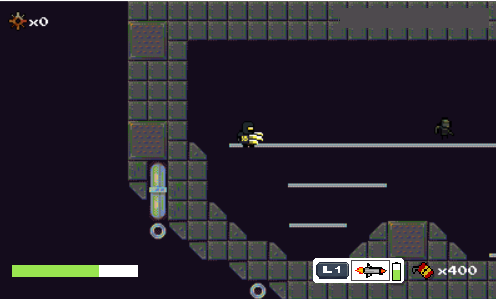
\includegraphics[width=\columnwidth]{Figures/HUD.png}
	\caption{HUD design (normally)}
\end{figure}


\begin{figure}[H]
	\centering
	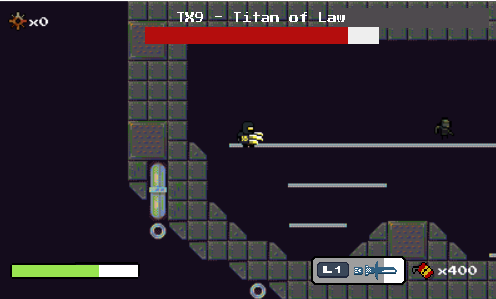
\includegraphics[width=\columnwidth]{Figures/HUDBoss.png}
	\caption{HUD design (active boss)}
\end{figure}

\subsubsection{Main Menu}

\begin{figure}[H]
	\centering
	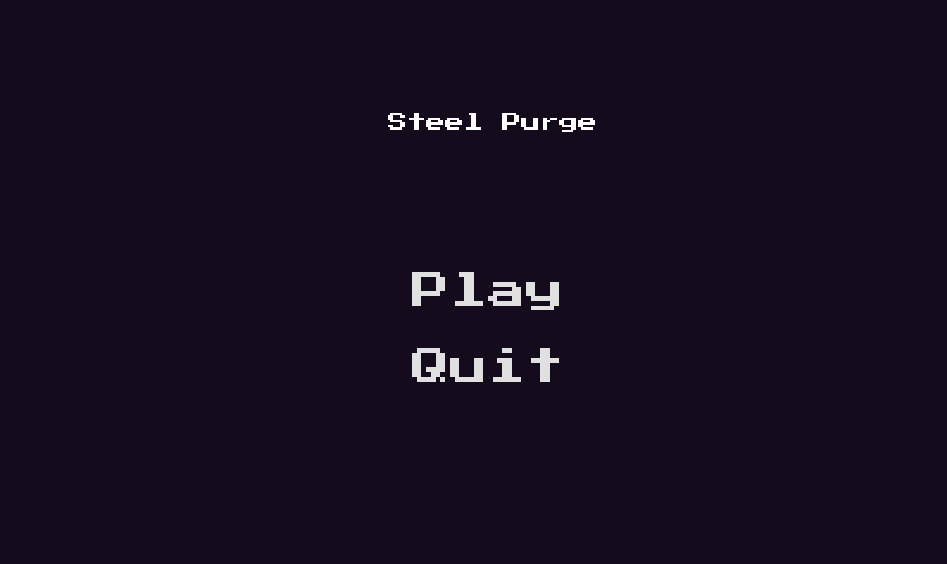
\includegraphics[width=\columnwidth]{Figures/StartMenu.png}
	\caption{Minimal viable main menu}
\end{figure}

\subsection{Game Art}

The art in Steel Purge will currently be purely pixel art. For Prototype 1, the art will consist of somewhat altered free pixel art ripped from itch.io. There will also exist some custom art for the relevant areas, such as weapons. The following list will show the required art elements:

\textbf{Player}
\begin{itemize}
	\item Jump
	\item Walk
	\item Run
	\item Sliding
	\item Shooting alternating between each hand
	\item All animations above with different weapons equipped
\end{itemize}

\textbf{Weapon Sprites (General)}
\begin{itemize}
	\item Item icon on ground
	\item Icon in inventory
	\item Ordinance icon on HUD
\end{itemize}


\textbf{Firewall}
\begin{itemize}
	\item Dragons breath fire jet stream
\item Flares
\item Burn effect on enemies 
\end{itemize}

\textbf{Joule}
\begin{itemize}
	\item Bubble shield sprite
	\item Kinetic orb 
	\item Orb explosion
\end{itemize}

\textbf{Neostar}
\begin{itemize}
	\item Slam player animation
	\item Slam impact sprite
	\item Magnetic energy orbs
\end{itemize}

\textbf{Rush Rogue}
\begin{itemize}
	\item Patrolling
	\item Detecting player
	\item Rushing player
	\item Death
\end{itemize}

\textbf{Executor}
\begin{itemize}
	\item Shooting player
	\item Running towards player
	\item Death
\end{itemize}

\textbf{Death Hornet X-08}
\begin{itemize}
	\item Walk
	\item Melee
	\item Spawn Rogue SIdeways
	\item Flight
	\item Spawn Rogue Airborne
	\item Downwards strike
	\item Rogue Mayhem
	\item Death
\end{itemize}

% \textbf{}
% \begin{itemize}
% 	\item 
% \end{itemize}

\subsection{Music}

The main menu and first level will have their own respective music themes. 

\subsection{Sound Effects}

The following list will indicate all the game elements that require a sound effect\newline

\textbf{Player:}
\begin{itemize}
	\item Jumping
	\item Sliding
	\item Taking damage
	\item Dying
	\item Walking
	\item Sprint start
	\item Collecting scrap
	\item Collecting fuels (both Gasoline and Energy is different)
	\item Health regeneration start
	\item Health regeneration cancel
	\item Health regeneration fill per tick
	\item Health regeneration end after full health
\end{itemize}

\textbf{Enemies in general}
\begin{itemize}
	\item Taking damage (and dropping scrap)
	\item Taking critical damage
	\item Dying (make robotic collapse sound)
\end{itemize}

\textbf{Rush Rogue}
\begin{itemize}
	\item Detecting Player
	\item Rushing Player
	\item Exploding on player
\end{itemize}

\textbf{Executor}
\begin{itemize}
	\item Firing rods
	\item Walking towards player
\end{itemize}

\textbf{Death Hornet X-08}
\begin{itemize}
	\item Walk
	\item Melee
	\item Spawn Rogue SIdeways
	\item Flight
	\item Spawn Rogue Airborne
	\item Downwards strike
	\item Rogue Mayhem
	\item Death
\end{itemize}

\textbf{Weapons}
\begin{itemize}
	\item When picked up (different for every weapon)
	\item Firing (different for every weapon)
	\item Ordinance used (different for every weapon)
	\item Ordinance ready
\end{itemize}

\textbf{Menus in general}
\begin{itemize}
	\item Button selection
	\item Button clicking
	\item Special button click (i.e, switching menu when pressed, crafting item in inventory)
\end{itemize}


\textbf{Inventory and Shop}
\begin{itemize}
	\item Open
	\item Close
\end{itemize}

\subsection{The first level}

\end{document}
